\newpage

\section{Вычислительный эксперимент}

Для анализа моделей, полученных путем дистилляции модели учителя в модель ученика, был проведен вычислительный эксперимент для задачи классификации.\\
\textbf{Выборка FashionMNIST.} Эксперимент проводился для выборки FashionMNIST~\cite{FMNIST} - набора изображений предметов одежды. В качестве моделей учителя $\textbf{f}$ и ученика $\textbf{g}$ рассматриваются четырёхслойная и однослойная нейронные сети соответсвенно, в качестве функции активации рассматривается ReLu. Градиентный метод оптимизации - Adam.\\
На рисунках 1, 2 показаны графики зависимостей accuracy и кросс-энтропии на тестовой выборке между истинными метками объектов и вероятностями, предсказанными моделью ученика. На графиках видно, что модель, использующая метки учителя, показывает лучшее значение Accuracy, при этом наблюдается незначительное повышение ошибки.

\begin{figure}[h!t]\center
\subfloat[]
{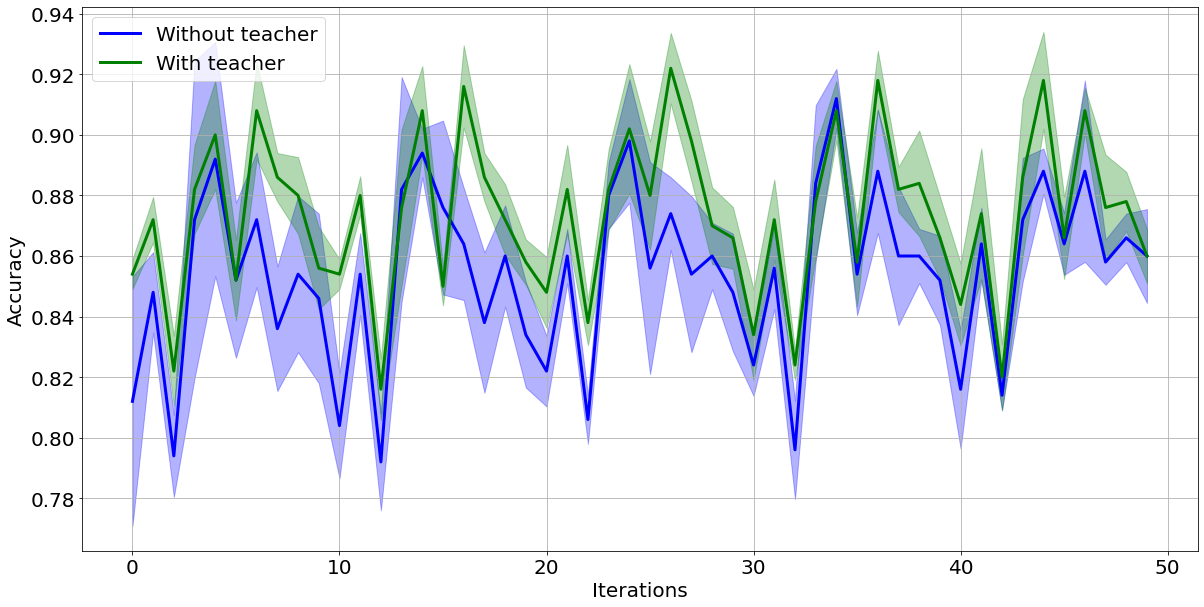
\includegraphics[width=0.5\textwidth]{results/accuracy}}
\subfloat[]
{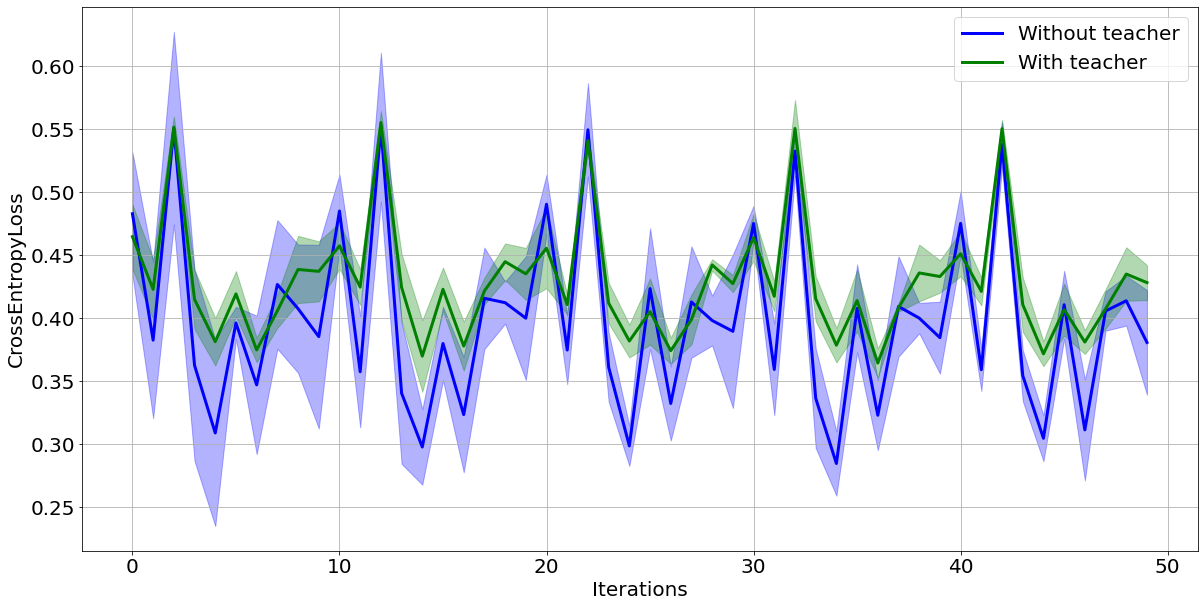
\includegraphics[width=0.5\textwidth]{results/loss}}\\
\caption{Зависимость a) Accuracy; b) CrossEntropyLoss между истинными и предсказанными учеником метками от числа итераций на тестовой выборке}
\end{figure}


\newpage
\subsection{Базовый экперимент}
